% Poster Figure 2 (Technical Approach, data): two-branch data curation.
% Adapted from Fig. data_pipeline in 3_method.tex. Sized for a 10.5in x 4.2in slot.
\documentclass[border=2pt]{standalone}
% Shared style for PRISM figures. Compile with tectonic (XeTeX engine).
\usepackage{lmodern}
\usepackage{amssymb}
\usepackage{fontspec}
\setmainfont{Arial}
\setsansfont{Arial}
\usepackage{amsmath}
\usepackage{booktabs}
\usepackage{colortbl}
\usepackage{xcolor}
\usepackage{tikz}
\usetikzlibrary{arrows.meta,positioning,fit,calc,backgrounds,decorations.pathreplacing}
\usepackage{pgfplots}
\pgfplotsset{compat=1.18}

% PRISM template palette (sampled from the poster template)
\definecolor{prismdark}{HTML}{195A99}
\definecolor{prismmid}{HTML}{1D6FAA}
\definecolor{prismlight}{HTML}{9BB7DC}
\definecolor{prismpale}{HTML}{E8EFF8}
\definecolor{prismaccent}{HTML}{D9822B}
\definecolor{prismgray}{HTML}{6B7280}

\newcommand{\sz}[2]{\fontsize{#1}{#2}\selectfont}
\newcommand{\oursrow}{\rowcolor{prismpale}}
\pgfkeys{/pgf/number format/assume math mode=true}

\begin{document}
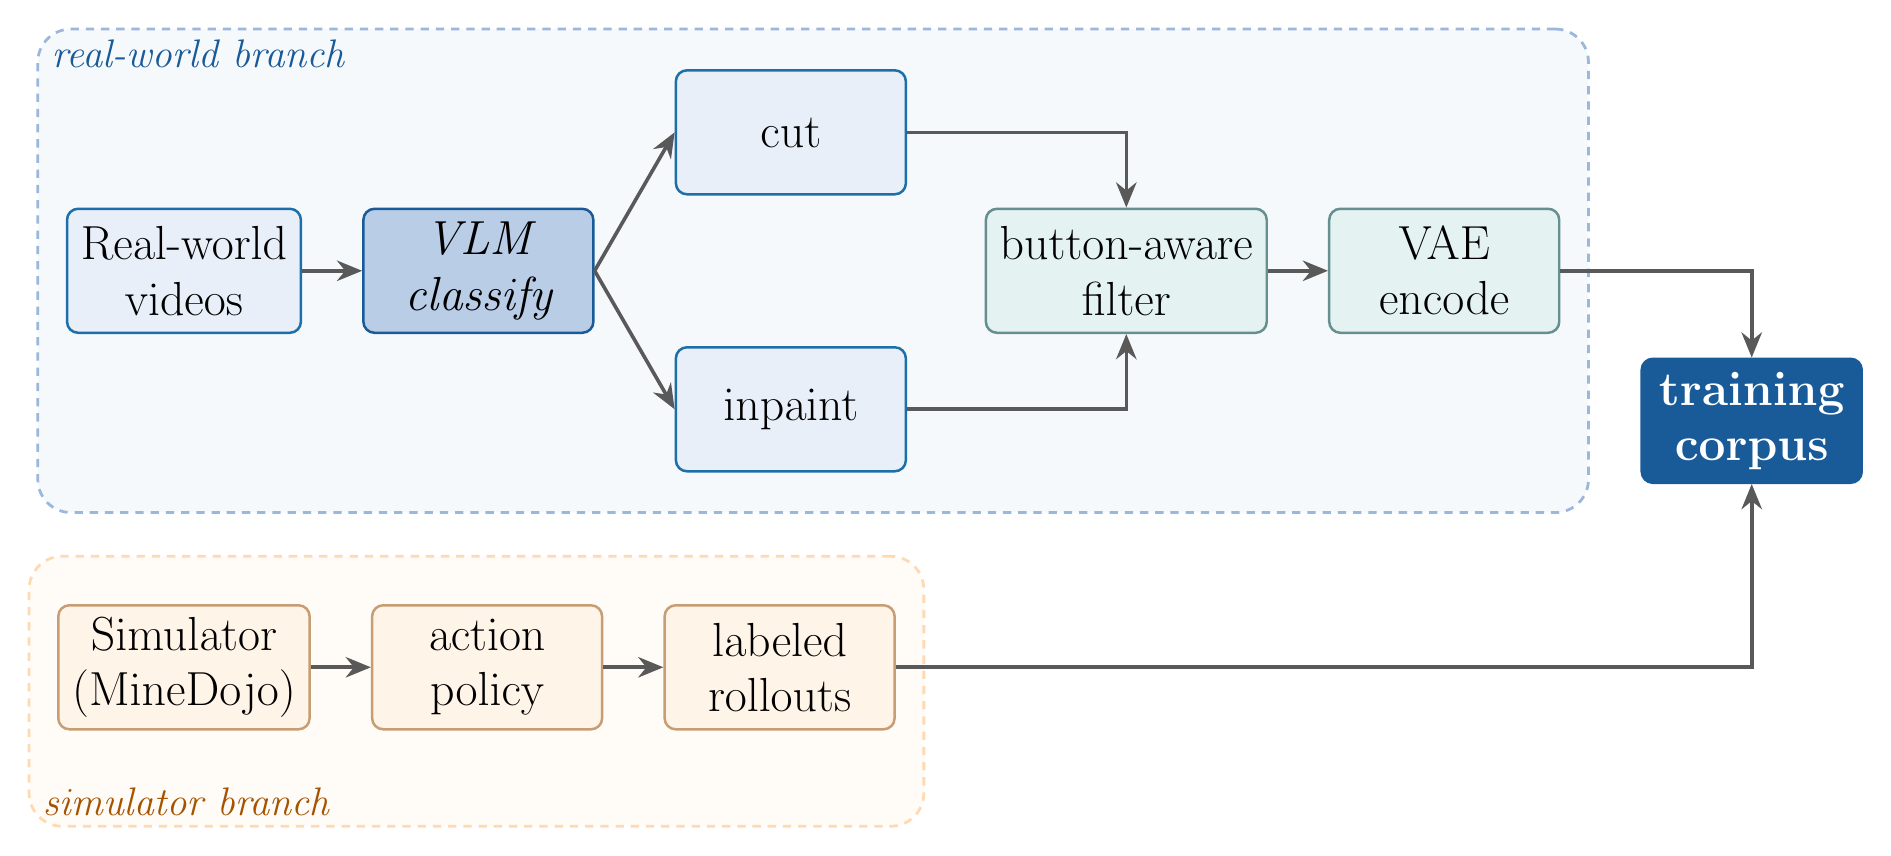
\begin{tikzpicture}[
    font=\sz{17}{20},
    >={Stealth[length=3.2mm,width=2.6mm]},
    proc/.style={
        rectangle, rounded corners=4pt, draw=black!55, line width=0.9pt,
        minimum height=0.62in, minimum width=1.15in,
        inner xsep=5pt, inner ysep=3pt, align=center, fill=white,
    },
    real/.style={proc, fill=prismpale, draw=prismmid},
    sim/.style={proc, fill=orange!9, draw=orange!60!black!55},
    decide/.style={proc, draw=prismdark, fill=prismlight!70, font=\sz{17}{20}\itshape},
    branch/.style={proc, fill=prismpale, draw=prismmid},
    shared/.style={proc, fill=teal!10, draw=teal!55!black!60},
    train/.style={proc, fill=prismdark, draw=prismdark, text=white, minimum width=1.1in, font=\sz{17}{20}\bfseries},
    arr/.style={->, line width=1.3pt, draw=black!65},
    node distance=0.22in and 0.3in,
]
\node[real] (data) {Real-world\\videos};
\node[decide, right=of data] (vlm) {VLM\\classify};
\node[branch, above right=0.06in and 0.4in of vlm] (cut) {cut};
\node[branch, below right=0.06in and 0.4in of vlm] (inp) {inpaint};
\node[shared, right=1.95in of vlm] (filter) {button-aware\\filter};
\node[shared, right=of filter] (vae) {VAE\\encode};

\node[sim, below=1.35in of data] (sim) {Simulator\\(MineDojo)};
\node[sim, right=of sim] (pol) {action\\policy};
\node[sim, right=of pol] (vid) {labeled\\rollouts};

\node[train, right=0.4in of vae, yshift=-0.75in] (train) {training\\corpus};

\draw[arr] (data) -- (vlm);
\draw[arr] (vlm.east) -- (cut.west);
\draw[arr] (vlm.east) -- (inp.west);
\draw[arr] (cut.east) -| (filter.north);
\draw[arr] (inp.east) -| (filter.south);
\draw[arr] (filter) -- (vae);
\draw[arr] (vae.east) -| (train.north);

\draw[arr] (sim) -- (pol);
\draw[arr] (pol) -- (vid);
\draw[arr] (vid.east) -| (train.south);

\begin{scope}[on background layer]
\node[fit=(data)(cut)(inp)(filter)(vae), rounded corners=12pt,
      fill=prismpale!40, draw=prismlight, line width=1pt, dash pattern=on 3pt off 2.5pt,
      inner xsep=0.14in, inner ysep=0.2in] (lane1) {};
\node[fit=(sim)(vid), rounded corners=12pt,
      fill=orange!3, draw=orange!30, line width=1pt, dash pattern=on 3pt off 2.5pt,
      inner xsep=0.14in, inner ysep=0.2in, yshift=-0.12in, minimum height=1.35in] (lane2) {};
\end{scope}
\node[anchor=north west, font=\sz{15}{18}\itshape, text=prismdark]
      at ([xshift=2pt,yshift=-1pt]lane1.north west) {real-world branch};
\node[anchor=south west, font=\sz{15}{18}\itshape, text=orange!65!black]
      at ([xshift=2pt,yshift=1pt]lane2.south west) {simulator branch};
\end{tikzpicture}
\end{document}
